\documentclass[a4paper,11pt,twocolumn]{article}
\usepackage{polyglossia} % Eesti keele tugi
\setdefaultlanguage{estonian}
\usepackage{geometry}% Paigutus
\usepackage{graphicx}% Joonised
\graphicspath{ {images/} }
\usepackage{csquotes}% Eesti jutumärgid \enquote{}
\usepackage{enumitem}% Listid
\usepackage[compact]{titlesec}% Kompaktsed pealkirjad
\usepackage{siunitx}% SI ühikud
\usepackage{tikz}
\usepackage[siunitx]{circuitikz}
\usepackage[final]{microtype}
\usepackage{amsmath}
\usepackage{lmodern}
\geometry{
    paper=a4paper, % Paper size, change to letterpaper for US letter size
    top=0.5cm, % Top margin
    bottom=1cm, % Bottom margin
    left=0.5cm, % Left margin
    right=0.5cm, % Right margin
    foot=0.5cm, % Footer-margin distance
    %showframe, % Uncomment to show how the type block is set on the page
}


%\setlength{\intextsep}{0pt}

\setlength{\parindent}{0cm}% Taandridu pole
\setlength{\parskip}{1em}% Paragraafide vahed
\setlist[itemize]{topsep=0em, partopsep=0em, parsep=0em, itemsep=0.5em}% Itemize spacing

\usepackage{xparse}

% Ülesanded \begin{question}[viide][joonis][joonise suurus] (võib olla ka ainult [viide] või [joonis][joonise suurus])
\newcounter{myproblems}
\NewDocumentEnvironment{question}{o o o}
{\par \refstepcounter{myproblems} \textbf{Ülesanne \themyproblems .} \ignorespaces\IfValueT{#1}{\IfValueTF{#3}{\textbf{(#1)} \ignorespaces}{\IfNoValueT{#2}{\textbf{(#1)} \ignorespaces}}}}
{\IfValueT{#2}{\IfValueTF{#3}{\begin{figure}[h!]\includegraphics[width=#3]{#2.pdf}\centering\vspace{-1em}\end{figure}}{\begin{figure}[h!]\includegraphics[width=#2]{#1.pdf}\centering\vspace{-1em}\end{figure}}}\ignorespacesafterend}

% Alaülesanded
\newenvironment{subquestion}
{\setlength{\parskip}{0pt}\begin{enumerate}[label=\alph*), nolistsep]}
{\end{enumerate}\setlength{\parskip}{1em}\ignorespacesafterend}

% Vihjete jaoks
\newenvironment{hint}[1][Vihje]
{\setlength{\parskip}{0em} \textit{#1}: \ignorespaces}
{\setlength{\parskip}{1em}\ignorespacesafterend}

\newcommand{\pvec}[1]{\vec{#1}\mkern2mu\vphantom{#1}}% Primed vector

% Lahendused jaoks
\usepackage{hyperref}
\newenvironment{solutions}
{\begin{enumerate}[label=\textbf{\arabic*.}, wide]}
{\end{enumerate}}

% Displaystyle valemite paigutus
\makeatletter
\g@addto@macro{\normalsize}{%
    \setlength{\abovedisplayskip}{4pt}
    \setlength{\abovedisplayshortskip}{4pt}
    \setlength{\belowdisplayskip}{4pt}
    \setlength{\belowdisplayshortskip}{4pt}
    }
\makeatother

% \directlua{dofile("DetectUnderfull.lua")}
\tikzset{
    odot/.style={
        circle,
        inner sep=0pt,
        node contents={$\odot$},
        scale=1
    },
    otimes/.style={
        circle,
        inner sep=0pt,
        node contents={$\otimes$},
        scale=1
    }}


\begin{document}
{\huge \textbf{Taevamehaanika} \hfill \normalsize{nr 9} \\
{Kaarel Kivisalu \hfill 2. aprill 2019}

\section{Taevamehaanika}
Kepleri seadused:
\vspace{-1em}
\begin{enumerate}
    \item Iga planeedi $a_1$ orbiit on ellips, mille ühes fookuses on Päike:
        \[
            r=\frac{p}{1+e \cos f}
        .\]
    \item Planeedi raadiusvektor katab võrdsete ajavahemike jooksul võrdsed pindalad:
        \begin{align*}
            \frac{\text{d} \vec{L}}{\text{d}t}&= \frac{d(\vec{r}\times m \vec{v})}{dt}= 0  \\
            \frac{\text{d} \vec{A}}{\text{d}t}&= \frac{1}{2}\frac{\vec{L}}{m}=\text{const}
        .\end{align*}
    \item Planeetide tiirlemisperioodide ruudud suhtuvad nagu nende orbiitide pikemate pooltelgede kuubid:
        \[
            P^2=\frac{4\pi^2}{G(m_1+m_2)}a^3
        .\]
\end{enumerate}

Newtoni gravitatsiooniseadus:
\[
F=\frac{Gm_1m_2}{r^2}
.\]
Energia orbiidil:
\[
E=K+P=\frac{mv^2}{2}-\frac{Gm_1m_2}{r}=-\frac{Gm_1m_2}{2a}
.\]
Runge-Lenz'i (ekstsentrilisuse) vektor:
\[
\vec{e}=\frac{\vec{v}\times \vec{L}}{Gm_1m_2}-\hat{r}=\text{const}
.\]
Orbiite on olemas kolme tüüpi: elliptilised, hüperboolsed ja paraboolsed.
\subsection{Ellips}
Ristkoordinaatides:
\[
\frac{x^2}{a^2}+\frac{y^2}{b^2}=1
.\]
Polaarkoordinaatides:
\[
r=\frac{p}{1+r \cos f}
.\]
$a$ on suur pooltelg, väike pooltelg $b=a\sqrt{1-e^2}$, $e$ on ektsentrilisus ($0\le e<1$), fookuse kaugus keskpunktist $c=ea$, poolfokaalparameeter $p=a(1-e^2)$, pindala $A=\pi ab$, energia $E<0$.
\begin{figure}[h!]
    \centering
    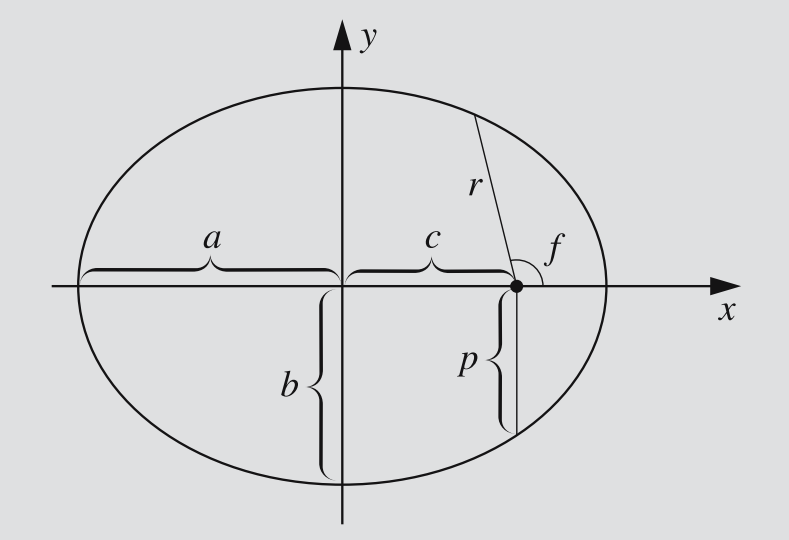
\includegraphics[height=4cm]{ast1.png}
    \label{fig:ast1-png}
\end{figure}

\subsection{Hüperbool}
Ristkoordinaatides
\[
\frac{x^2}{a^2}-\frac{y^2}{b^2}=1
.\]
Polaarkoordinaatides:
\[
r=\frac{p}{1+e \cos f}
.\]
Ekstsentrilisus $r>1$, väike pooltelg $b=a\sqrt{e^2-1}$, poolfokaalparameeter $p=a(e^2-1)$, asümptoodid $y=\pm \frac{b}{a}x$, energia $E>0$.
\begin{figure}[h!]
    \centering
    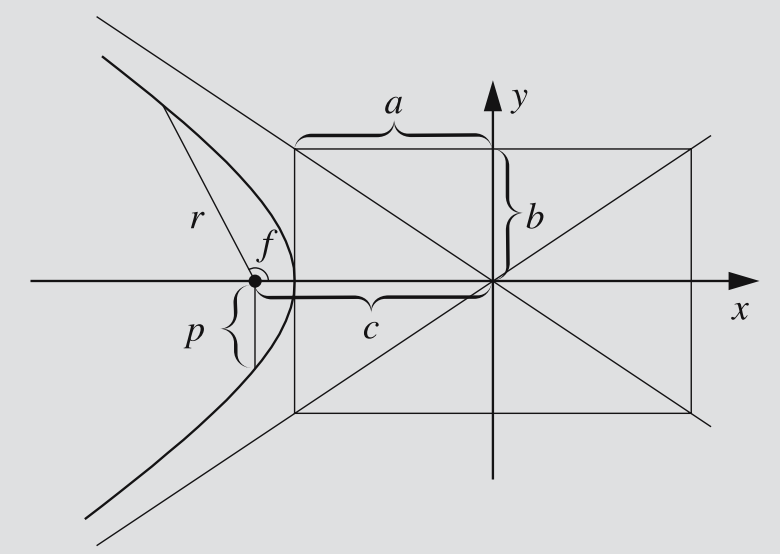
\includegraphics[height=4.2cm]{ast2.png}
    \label{fig:ast2-png}
\end{figure}

\subsection{Parabool}
Ristkoordinaatides:
\[
x=-ay^2
.\]
Polaarkoordinaatides:
\[
r=\frac{p}{1+e \cos f}
.\]
Ekstsentrilisus $e=1$, poolfokaalparameeter  $p=\frac{1}{2}a$, $h=\frac{1}{4}a$, energia $E=0$.
\begin{figure}[h!]
    \centering
    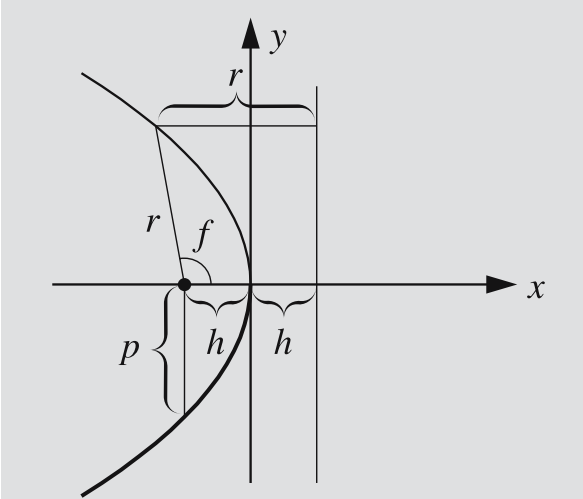
\includegraphics[height=5cm]{ast3.png}
    \label{fig:ast3-png}
\end{figure}
\vspace{-1em}

\subsection{Ülesanded}

\begin{question}
    Leidke ringorbiidil raadiusega $R=R_M$ liikumise periood, kus $R_M$ on Maa raadius.
\end{question}

\begin{question}
    Leidke aeg, mis kulub Maa sisse kaevatud tsentrit läbiva tunneli kaudu \enquote{kukkumiseks} teisele poole Maakera.
    \begin{hint}
    Vihje: kiirenduse sõltuvus koordinaadist peaks tulema harmoonilise ostsillaatoriga samal kujul $a=-\omega^2x$. Võrrelge seda aega esimese kosmilise kiirusega Maa ümber tiiru tegemise ajaga. Kas tulemus oleks teine, kui see tunnel ei läbiks Maa keskpunkti?
    \end{hint}
\end{question}

\begin{question}
    Tõestage, et kui planeedi sisemusse teha sfääri-kujuline õõnsus, siis selle sees on väli homogeenne.
\end{question}

\begin{question}
    Tuletage koguenergia (kineetiline pluss potentsiaalne) avaldis
    \[
    E=-\frac{Gm_1m_2}{2a}
    .\]
\end{question}

\begin{question}
    Maapinnalt visatakse vertikaalselt üles mingi objekt sellise kiirusega, et see eemaldub Maast kaugusele $R$ ning tuleb siis tagasi. Leidke objekti lennu-aeg. Maa raadius on $R_M=R$.
\end{question}

\begin{question}
    Objekt saadetakse orbiidile kahes etapis: esmalt antakse maapinna läheduses kiirus $v_2$ ning apogees suurendatakse kiirust: $v_2=v+\Delta v$ nii, et objekt on nüüd ringorbiidil raadiusega $R$, Maa raadius on $R_M$. Leida $v_1$ ja $\Delta v$.
\end{question}

\begin{question}
   Ringorbiidil $R$ objektile antakse radiaalsuunaline kiirus. Kui suur peab see kiirus olema, et objekt väljuks Maa orbiidilt? Maa raadius on $R_M$.
   \begin{hint}
       Milline peab olema objekti koguenergia, et väljuda orbiidilt (liikuda lõpmatult kaugele)?
   \end{hint}
\end{question}

\begin{question}
    Mingi tähe läheduses toimub plahvatus, kust lendab välja palju väikseid objekte, kõigi kiiruste moodulid on võrdsed $v$-ga. Objektid hakkavad liikuma elliptilisi orbiite mööda, mille üheks fookuseks on see täht. Kus võib aga asuda teine fookus? (Leidke teise fookuse geomeetriline koht.)
\end{question}

\begin{question}[Tudengite olümpiaad 2003]
    Vaadelgem tähtedevahelise gaasipilve gravitatsioonilist kokkutõmbumist. Eeldagem, et gaas tihedusega $\rho=\SI{10e-15}{kg.m^{-3}}$ täidab ühtlaselt kerakujulise ruumiosa ning algtemperatuur on nii madal, et osakeste algkiiruse võib lugeda nulliks. Kui kaua võtab aega gaasipilve kokkutõmbumine?
\end{question}

\begin{question}[ast4][0.9\columnwidth]
    Lõpmatusest läheneb tähele mingi objekt ning eemaldub seejärel taas lõpmatusse. Lõpmatult kaugel olles on kiirusvektori poolt moodustatd sirge kaugus tähest $b$ (vt joonist), pärast eemaldumist on sama parameeter $b'$ (milline on seos nende vahel?). Leidke avaldis kõrvalekalde-nurga $\phi$ jaoks.
    \begin{hint}
        Runge-Lenz'i vektor võib osutuda kasulikuks.
    \end{hint}
\end{question}

\end{document}
